\chapter{State of Art}
\label{chapter:state_of_art}

\section{Manually Managing \acl{lf} Items} \label{sec:manually-managing-lf-items}

\subsection{Traditional Management Systems} \label{subsec:traditional-lf-systems}

Traditional \acp{lfms} typically relied on manual processes to log and manage items, sometimes papers or books and, in a few cases, spreadsheets \cite{Anas2023}. The fundamental components included physical logs, where details of found items - such as descriptions, location, and date of discovery - were recorded by staff or custodians.

Often, the responsibility of maintaining these records fell to a designated individual or department. Items were categorised and stored in a secure area, with the hope that owners would reclaim them. Matching found items to reported losses was a manual process, requiring significant time and effort \cite{Anas2023}. Descriptions provided by claimants were cross-referenced with recorded details to determine ownership. In some cases, rudimentary tagging systems were used to label items, aiding the identification process.

In environments like universities or corporate campuses, basic digital tools such as spreadsheets were usually introduced to track items. However, the overall workflow remained heavily dependent on manual oversight. Community bulletin boards, notices, or word-of-mouth were also standard methods to inform individuals about found items.

Despite their simplicity, these systems played a critical role in facilitating the return of lost belongings in the pre-digital era \cite{Mayura2024}. They fostered a sense of trust and collaboration within communities, relying on the goodwill and honesty of both finders and administrators. The traditional systems established the groundwork for modern approaches, providing valuable insights into the challenges and requirements of effective \ac{lf} management.

Despite the previously detailed inefficiencies of such systems, there are still those who would find these manual workflows to be more trustworthy. For some, the human element brings a level of accountability and understanding that automated systems cannot replicate. Manual processes allow for subjective judgment, which can be beneficial in complex scenarios where nuance is required. The tactile nature of handling paper documents or physical records fosters a sense of security and reliability. Moreover, people who have had negative experiences with technology might prefer traditional methods, viewing them as more stable and less prone to glitches or failures.


\subsection{Obstacles in Traditional Systems} \label{subsec:obstacles-traditional-systems}

While traditional \acp{lfms} have historically served their purpose in smaller or less demanding contexts, they face significant challenges when scaled to handle larger volumes of items or more complex environments \cite{Mayura2024}. The scalability of such systems is inherently constrained by their reliance on manual processes and both limited technological integration and automation.

A key obstacle is the dependency on human effort. As the number of items increases, so does the burden on staff, leading to delays, errors, and inefficiencies. In high-traffic environments, the sheer volume of items can quickly overwhelm even the most organised traditional systems. Without automation, processing and resolving claims becomes a time-intensive task, reducing the workflow's overall effectiveness. 

Another barrier to scaling is the lack of centralised data management. In traditional systems, records are often siloed, with each location or department maintaining its logs. Especially in larger organisations or distributed campuses, the absence of a unified database also impedes efficient reporting and analysis of trends, such as identifying frequent loss locations or categories of items.

Communication between stakeholders presents further challenges. Traditional systems often lack any mechanisms for notifying individuals about found items or updating claimants on the status of their reports, resulting in inefficiencies and frustrations, particularly in large-scale operations where the number of inquiries can be substantial.

Finally, the security of manual systems poses significant concerns. As the volume of items increases, the risk of theft, loss, or unauthorised access also rises. Inadequate labelling and verification processes can lead to disputes or errors in returning items to their rightful owners, further eroding trust in the system.

% These obstacles highlight traditional systems' limitations in adapting to the demands of modern \ac{lf} management. While effective in smaller, community-focused settings, their scalability issues underscore the need for innovative solutions that leverage technology to enhance efficiency, security, and user satisfaction.


\section{Inventory Management Systems} \label{sec:ims}

\acp{ims} are tools designed to manage and track inventory levels across various domains. These systems enable organisations to streamline their operations, reduce costs, and enhance customer satisfaction by ensuring the availability of necessary items at the right time and place \cite{Pauliina2024}. An \ac{ims} employs methodologies to identify and classify inventory items based deatails like quantity, volume, value or variability, optimising inventory performance through targeted strategies \cite{Pauliina2024}.

Fundamentally, an \ac{ims} aims to address some challenges, such as maintaining inventory levels, reducing holding costs, mitigating risks and many others associated with collections and stocks. Techniques like safety stock determination and lot-sizing methods have been widely adopted \cite{Prabakaran2023}. Such systems have historically evolved to incorporate some technological advancements, obtaining the capability to predict, plan, and execute inventory operations Automatically and effectively \cite{Chebet2019}.

While conventional \acp{ims} primarily focus on physical products, their underlying principles can be effectively applied to tracking and managing \ac{lf} items. This intersection becomes particularly relevant in environments where the inventory (in this case, lost items) exhibits variability in value, volume, and retrieval demand. Inventory management principles, such as classification and optimisation, can be applied to \acp{lfms} to streamline processes and enhance user experiences. For instance, using the classification method mentioned before, in a \ac{lfms}, items could be categorised using an adapted ABC-XYZ\footnote{Suryaputri Z. and Gabriel, D.S. and Nurcahyo R., Integration of ABC-XYZ Analysis in Inventory Management Optimization: A Case Study in the Health Industry, Proceedings of the International Conference on Industrial Engineering and Operations Management, 2020, \url{https://ieomsociety.org/proceedings/2022nigeria/70.pdf}}framework that enables prioritisation of storage, retrieval, and notification efforts \cite{Khobragade2018}. The Table \ref{tab:abc_xyz} illustrates a potential result of that association:

\begin{table}[H]
\centering
\caption{Classification of \ac{lf} items using the ABC-XYZ framework}
\begin{tabular}{|c|c|c|c|c|}
\hline
\textbf{Class} & \textbf{Value} & \textbf{Volume} & \textbf{Retrieval Demand} & \textbf{Examples} \\ 
\hline
A-X & High & Low & Consistent & Electronic devices, jewellery \\ 
\hline
B-Y & Moderate & Moderate & Fluctuating & Wallets, bags, clothing \\ 
\hline
C-Z & Low & High & Irregular & Umbrellas, stationery \\ 
\hline
\end{tabular}
\label{tab:abc_xyz}
\end{table}

The insights from \citeauthoryear{Plinere2016} further support the integration of these methodologies into \acp{lfms}. Their case study emphasises the significance of structured inventory management practices for improving operational efficiency. For instance, high-priority items, such as class A-X items, can benefit from focused attention and expedited claim processes, ensuring user satisfaction while reducing storage costs. Furthermore, their findings highlight the value of predictive analytics in addressing slow-moving or stagnant inventory, matching to unclaimed items \cite{Plinere2016}. Technological integration, as illustrated in the case study, offers another avenue for improvement. The use of \ac{rfid} and \ac{qr} codes in conventional inventory systems ensures accurate tracking and categorisation of items \cite{Plinere2016, Sohail2018}. Moreover, the adoption of resource planning principles, such as imposing a centralised warehouse, would improve transparency and decision-making, possibly enabling a seamless synchronisation of data across departments. Lastly, the \citeauthoryear{Plinere2016} study underlines the importance of standardisation in inventory management policies, e.g., uniform intake procedures, categorisation standards, and clear guidelines for item disposition.

Adapting \acp{ims} for \ac{lf} management would definitely address some unique challenges \cite{Pauliina2024}. Unlike traditional inventory, lost items often have sentimental value or urgent retrieval needs, requiring the system to incorporate real-time tracking and user-friendly interfaces. Moreover, integrating predictive analytics, commonly used in \acp{ims} for forecasting demand, would be leveraged to anticipate peak periods of item loss or retrieval, e.g., events or seasons that may influence the volume and types of items lost, allowing proactive resource allocation \cite{Prabakaran2023}.

Building on these foundational principles, open-source \acp{ims} have evolved to address specific needs, blending traditional methodologies with modern technologies to enhance their adaptability and utility across domains. Odoo Inventory\footnote{\url{https://www.odoo.com/app/inventory}}, for instance, exemplifies this progression by integrating inventory management with enterprise-level tools like sales and customer relationship management. Its multi-warehouse support and barcode scanning capabilities make it a robust solution for medium to large enterprises. In contrast, Snipe-IT\footnote{\url{https://snipeitapp.com/demo}} focuses on a narrower domain (asset tracking), offering a well-designed interface for managing fixed assets, albeit without features like demand forecasting or multi-warehouse management. Moving further into specialised territories, InvenTree\footnote{\url{https://inventree.org/}} demonstrates how inventory systems can cater to engineering and manufacturing by providing tools for managing parts and components through hierarchical structures and batch tracking. However, it lacks the scalability offered by integration with other systems. Meanwhile, SkuNexus\footnote{\url{https://skunexus.com}} exemplifies the pivot toward e-commerce needs, combining advanced reporting, omnichannel order fulfilment, and process automation for complex operations, though its configurability demands significant effort during implementation. For small-scale, niche applications, PartKeepr\footnote{\url{https://partkeepr.org/}} offers essential inventory management tools, such as batch tracking and stock alerts, tailored to managing electronic components but without the scalability or advanced features needed for more extensive operations.

The following Table \ref{tab:ims_comparison} summarises the key features of these systems, highlighting their areas of strength and limitations:

\begin{table}[!htb]
\centering
\caption{Summarised comparison of open source \acl{ims} by features}
\begin{tabular}{lllllll}
\hline
\textbf{\ac{ims}} & \textbf{MWS} & \textbf{BI} & \textbf{DF} & \textbf{BT} & \textbf{ERPI} & \textbf{UFI} \\
\hline
Odoo & Yes & Yes & Yes & Yes & Yes & Yes \\
\hline
Snipe-IT & No & No & No & No & No & Yes \\
\hline
InvenTree & No & Yes & No & Yes & No & Yes \\
\hline
SkuNexus & Yes & Yes & Yes & Yes & Yes & No \\
\hline
PartKeepr & No & Yes & No & Yes & No & No \\
\hline
\end{tabular}
\caption*{\\MWS - Multi-Warehouse Support, BI - Barcode Integration, DF - Demand Forecasting, BT - Batch Tracking, ERPI - ERP Integration, UFI - User-Friendly Interface.}
\label{tab:ims_comparison}
\end{table}


\section{\acl{slr}} \label{sec:literature-review}

\subsection{Research Question and Methods} \label{subsec:slr}

\ac{lf} management has historically presented numerous challenges across both public and private sectors, as highlighted in a wealth of academic articles and studies \cite{Prawira2024}. To address previously mentioned persistent issues and uncover effective solutions, a rigorous \ac{slr} was undertaken, focusing specifically on innovations, challenges, and best practices in the realm of intelligent lost property management. The review was designed with a methodological rigour that adheres to the PRISMA 2020 guidelines \cite{Page2021}, ensuring that every aspect of the research was conducted with the highest standards of integrity and transparency. By synthesising the latest uncovered findings, the \ac{slr} offers not only a comprehensive understanding of the current landscape but also valiable insights that can inform the design of a \ac{lfms} system. The \ac{slr} later resulted in the production of a document directly aligned with this dissertation's scope, named \textit{"Designing an Intelligent Solution for Lost Property Management: A Systematic Review"}.

The review sought to answer the central research question \textit{"How can intelligent technologies enhance the efficiency and user experience of lost property management systems?"}, which refers to how technologies such as \ac{ai}, \ac{nlp}, \ac{cv} and many others can provide solutions to the inefficiencies in \ac{lf} management. The \ac{slr} analysed numerous articles and integrated 18 high-quality studies that demonstrated the capacity to provide new insights into the investigation area. The mentioned research question was then separated into the following three major objectives:

\begin{itemize}
\item Evaluating the applicability of the selected technologies;
\item Examining existing challenges in implementing these technologies;
\item Identifying best practices to inform the design and development of a proposed system.
\end{itemize}

The \ac{slr} employed a comprehensive four-phase approach, associated with the selected PRISMA framework. During the identification phase, academic databases such as Scopus and Web of Science were queried using targeted keywords like \ac{lf} Management, \ac{ims}, \ac{ai}, \ac{nlp}, and \ac{llm}, resulting in an initial yield of 476 studies. These were screened for relevance through the removal of duplicates and an abstract examination. In the eligibility phase, full-text articles were meticulously assessed against predefined inclusion criteria, which focused exclusively on studies published between 2020 and 2024 that addressed ac{ai}-based solutions. Non-peer-reviewed works and studies lacking empirical validation were excluded. Additionally, to ensure the robustness of the \ac{slr}, a quality assessment framework evaluated the methodological rigour and relevance of each study. Each study was rated on its technological contributions and practical applicability. Only those scoring consistently high across all criteria were included. Ultimately, in the inclusion phase, 18 studies were selected and categorised based on the technologies employed. Figure \ref{fig:prisma} illustrates the PRISMA flowchart, summarising the selection process. A thematic analysis was conducted, extracting valuable results into the contributions of each technological domain.

\begin{figure}[!htb]
    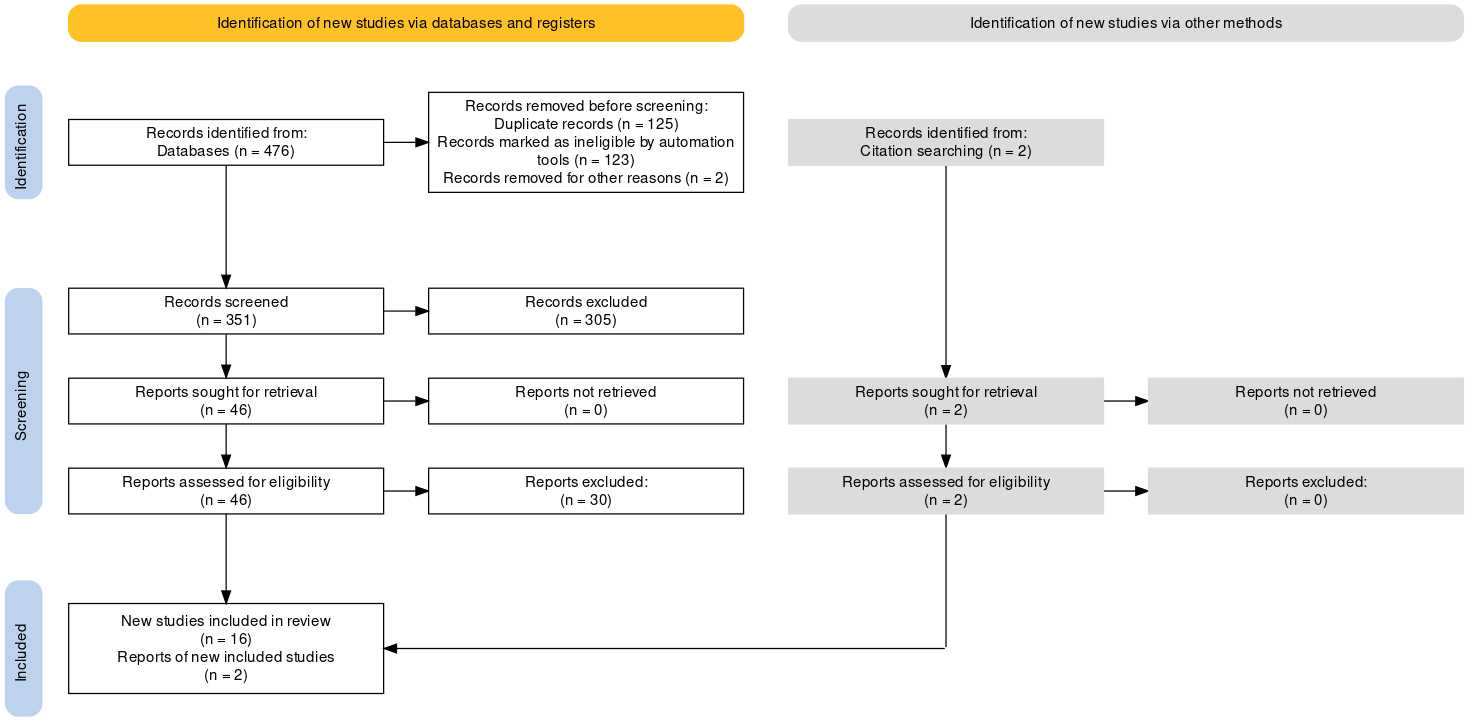
\includegraphics[width=0.95\textwidth]{figs/chapter2/prisma.png}
    \centering
    \caption[PRISMA flow diagram with a described quantity of research in each step.]{PRISMA flow diagram with a described quantity of research in each step.}
    \label{fig:prisma}
\end{figure}

\subsection{Object Recognition and Categorisation} \label{subsec:object-recognition}

Object recognition and categorisation are pivotal processes in the domain of \ac{ai} and \ac{cv}. Object recognition involves identifying objects within an image or video and distinguishing them based on predefined features. Categorisation goes a step further by grouping identified objects into classes and/or groups of classes based on shared attributes or relationships \cite{Liu2021}. These tasks are foundational to numerous applications, including autonomous vehicles, facial recognition, surveillance systems, and many others.

The origins of object recognition can be traced back to the early experiments in pattern recognition during the 1950s and 1960s. Early approaches relied heavily on rule-based systems, where objects were identified using manually defined features such as edges, corners, or textures. \citeauthoryear{Marr1982}'s seminal work on computational vision in the 1980s introduced the concept of multi-level processing, exposing the importance of integrating both low-level (e.g., edge detection) and high-level (e.g., semantic) features. The field evolved significantly in the 1990s with the advent of statistical methods and \ac{ml}. Techniques like support vector machines and decision trees provided more robust frameworks for categorisation \cite{Bishop2006}. Concurrently, datasets such as MNIST\footnote{\url{https://yann.lecun.com/exdb/mnist/}} and ImageNet\footnote{\url{https://www.image-net.org/}} emerged, enabling standardised benchmarking and driving advancements in recognition accuracy.

The evolution of object recognition and categorisation has been marked by the rise of \ac{dl} in the 2010s. \acp{cnn}, such as AlexNet\footnote{\ac{cnn} architecture, designed by Alex Krizhevsky in collaboration with Ilya Sutskever and Geoffrey Hinton at the University of Toronto in 2012} and \ac{resnet}, models capable of leveraging feature extraction, revolutionised this field by achieving human-like performance on challenging tasks. These models finally enabled the recognition of complex patterns and relationships in data \cites{He2015, Krizhevsky2017}. More recently, transformer-based architectures, exemplified by vision transformers, have further enhanced the capabilities of recognition systems. These models utilise attention mechanisms to capture long-range dependencies and contextual information, surpassing the limitations of traditional \acp{cnn} \cite{Dosovitskiy2020}.

\acp{cnn}, particularly \ac{resnet}-50, are widely utilised due to their capability to extract robust visual features. Studies have shown that ResNet-50 achieves high accuracy in identifying objects with varying attributes and appearances, a critical aspect for handling the heterogeneity of \ac{lf} items such as electronics, accessories, or apparel \cites{Prawira2024, Ghazal2016, Liu2022}. Similarly, \ac{yolo} models, including \ac{yolo}v7, are renowned for their real-time detection capabilities, ensuring low-latency processing and high precision even in challenging environments such as low light or cluttered backgrounds \cites{Sharma2024, Vedanth2024}.

\ac{resnet}-50, short for \acl{resnet} with 50 layers, has a \ac{dl} architecture designed to address the vanishing gradient problem in very deep neural networks. It introduces shortcut connections, or residual blocks, that allow gradients to flow more effectively during backpropagation, ensuring better convergence during training. \ac{resnet}-50 has become a standard in computer vision tasks due to its balance of depth and computational efficiency, making it suitable for extracting intricate visual features from diverse datasets \cite{He2015}. Its ability to generalise across object categories makes it a reliable choice for \ac{lf} management applications. \ac{yolo} is an object detection algorithm known for its speed and accuracy. Unlike traditional methods that scan an image region by region, \ac{yolo} processes the entire image in a single pass, predicting bounding boxes and class probabilities simultaneously, which significantly reduces computation time while maintaining high detection precision. \ac{yolo}v7, a more recent iteration, builds on these strengths by introducing architectural improvements for better performance in real-time scenarios, including high-density environments like traffic monitoring \cites{Redmon2015, Wang2022}.

Object recognition models can struggle with computational intensity, requiring significant resources for training and deployment \cites{Lubna2021, Mezhenin2021}. Lightweight versions of models are being developed to mitigate these issues, particularly for mobile applications, which are essential for systems designed to be universally accessible. Mobile-compatible frameworks, using optimised \ac{cnn}, provide the added advantage of enabling real-time item reporting and retrieval through user-friendly interfaces, expanding the reach of such systems \cites{Stout2024, Ghazal2016}.

Furthermore, these systems still need to contend with the diverse characteristics of objects. Items with subtle features or ambiguous shapes often pose difficulties for detection algorithms. Addressing this requires extensive and diverse datasets for training and validating in order to ensure that models can generalise effectively without overfitting to specific item categories \cites{Prawira2024, Liu2022, Sharma2024}. Hybrid approaches that integrate multiple algorithms or modalities are emerging as strategies to overcome these limitations. For instance, combining cloud-based data synchronisation with multimodal recognition has improved retrieval rates by facilitating large-scale processing and analysis \cite{Liu2024, Vedanth2024}.

\subsection{\acl{nlp}} \label{subsec:nlp}

\ac{nlp} is a multidisciplinary field at the intersection of linguistics, computer science, and artificial intelligence, enabling machines to process, understand, and generate human language. \ac{nlp} encompasses two core subfields: \ac{nlu} and \ac{nlg} \cite{Khurana2023}. \ac{nlu} focuses on interpreting and extracting meaning from textual or spoken language, including tasks such as sentiment analysis, intent recognition, and entity extraction, allowing systems to comprehend user input and respond accordingly \cite{Khurana2023}. In contrast, \ac{nlg} involves creating coherent and contextually appropriate textual or spoken output from structured data, such as generating summaries, reports, or conversational responses \cite{Dong2021}.

The origins of \ac{nlp} date back to the 1950s, when \citeauthoryear{Turing1950} proposed the concept of machine intelligence in his seminal work "Computing Machinery and Intelligence". One of the early milestones was the development of the Georgetown-IBM experiment in 1954, which demonstrated automatic translation between Russian and English, albeit limited to a small vocabulary and specific grammatical constructs. This marked the beginning of using computers to process and understand human language \cite{Hutchins2004}. About 50 years later, in the 1990s and early 2000s, \ac{ml} algorithms, mainly supervised learning, began to dominate \ac{nlp}, enhancing part-of-speech tagging, named entity recognition, and sentiment analysis. This era also witnessed the rise of the first large-scale resources for \ac{nlp}, including the Penn Treebank\footnote{https://catalog.ldc.upenn.edu/docs/LDC95T7/cl93.html} and WordNet\footnote{https://wordnet.princeton.edu/}, which provided valuable training data and lexical knowledge \cite{Marcus1993, Fellbaum1998}.

More recently, the new era has been characterised by a revolution in \ac{nlp} fueled by \ac{dl}. Neural network architectures, particularly recurrent neural networks and their derivatives, long short-term memory networks, demonstrated remarkable capabilities in sequence-to-sequence tasks such as translation and text summarisation \cite{Bahdanau2015}. Furthermore, the introduction of attention mechanisms and transformer-based models, such as \ac{bert} and \ac{gpt}, has drastically improved the state of the art, enabling unprecedented performance across a wide range of \ac{nlp} tasks \cite{Vaswani2017, Devlin2019}. Today, \ac{nlp} continues to evolve, integrating cutting-edge advancements in \ac{ai}, including transfer learning and pre-trained language models, to achieve higher accuracy and efficiency in a variety of complex tasks, namely sentiment analysis, machine translation, and conversational agents \cite{Howard2018}.

The systematic review highlights the growing role of \ac{nlp} in intelligent systems, particularly in enhancing human-computer interaction and automating complex processes. For instance, \ac{nlu} is central to enabling systems to interpret user input, extracting key entities, sentiments, and intents. \citeauthoryear{Prawira2024} and \citeauthoryear{Ghazal2016}, have already adopted these capabilities in their \ac{lfms} to streamline the reporting and retrieval of lost items. By leveraging \ac{nlu} models, their systems can process user descriptions into structured data that, once properly stored and indexed, can later be matched against found items.

Despite these advancements, several challenges remain. Scalability and computational efficiency are ongoing concerns, particularly when deploying \ac{nlp} models in real-time applications. Additionally, ethical considerations, including bias in language models and data privacy, require attention to ensure the responsible use of \ac{nlp} technologies \cite{Prawira2024}.


\subsection{Multimodal Matching} \label{subsec:multimodal-matching}

Embeddings play a pivotal role in modern artificial intelligence, particularly for applications requiring the integration of multimodal data such as images and text. These embeddings transform high-dimensional data into a lower-dimensional vector space while preserving semantic relationships. For example, image embeddings are often generated using \ac{cnn}, whereas text embeddings leverage transformer-based models \cite{He2015, Devlin2019}. This dimensionality reduction enables efficient and meaningful comparisons across large datasets.

Similarity search is a cornerstone technique in embedding-based systems. \citeauthoryear{Prawira2024} and \citeauthoryear{Ghazal2016} have experimented with metrics such as cosine similarity and Euclidean distance in order to quantify the proximity between embeddings, offering probabilistic measures of match likelihood between simulated \ac{lf} items. A high cosine similarity score, for instance, suggests strong alignment between query and database entries. Probabilistic models can further refine these measures, incorporating confidence intervals that guide the decision-making \cite{Dosovitskiy2020}.

Considering the domain of \ac{lf} management, embeddings would facilitate the matching of user-provided data to stored items or records. Visual embeddings derived from processed uploaded images would be compared against a database of known items. Similarly, textual embeddings generated from user descriptions and interactions could be matched to metadata or textual entries in the database. When combined, these approaches improve the accuracy and robustness of the matching process \cite{Prawira2024, Radford2021}. For instance, the integration of image and text embeddings through models like \ac{clip} enables effective multimodal matching by aligning visual and textual information in a unified vector space \cite{Radford2021}.

On the one hand, embedding-based systems face challenges related to scalability, bias, and computational demands. Scaling these systems to handle large datasets requires optimisation techniques such as lightweight models or distributed computing \cite{Lubna2021}. Moreover, biases inherent in pre-trained models can affect fairness, mainly when embeddings are derived from imbalanced datasets \cite{Prawira2024}. On the other hand, despite these challenges, empirical studies underscore the efficacy of multimodal matching in \acp{lfms}. For instance, \citeauthoryear{Prawira2024} achieved a 97.92\% matching accuracy by integrating \ac{resnet} embeddings with cosine similarity. \citeauthoryear{Ghazal2016} demonstrated an 89.2\% retrieval accuracy using a multi-feature image matching approach that incorporated texture, shape, and colour features.

% \subsection{Privacy and Security} \label{subsec:privacy-security}

% Todo: Write this section.

% \subsection{User Experience} \label{subsec:user-experience}

% Todo: Write this section.

% \subsection{Gamification} \label{subsec:gamification}

% Todo: Write this section.


\section{In-Production \acl{lfms}} \label{sec:in-production-solutions}

The management of \ac{lf} items has evolved over the years, resulting in modern \acp{lfms} that leverage innovative features. This section delves into some of the most prominent \acp{lfms}, grouped by their functionality and strengths. All the systems that are going to be explored combine with integrated shipping and return subsystems, which expresses the importance of this feature in the context of \ac{lf} management.

\subsubsection{Comprehensive and Feature-Rich Solutions} \label{subsubsec:comprehensive-solutions}

NotLost\footnote{\url{https://notlost.com}} stands out as a highly versatile \ac{lfms}, offering a broad array of features that make it suitable for organisations of all sizes. Its robust automated matching and search capabilities, powered by some rudimentary artificial intelligence, simplify item identification and matching processes. The platform also emphasises data security and compliance, but despite its many strengths, NotLost lacks features for disposal and recycling, leaving room for improvement in managing unclaimed items.

Similarly, Chargerback\footnote{\url{https://www.chargerback.com}} offers an extensive feature set comparable to NotLost, with added emphasis on reporting and analytics and disposal and recycling management, making it an ideal choice for organisations that require comprehensive reporting tools to analyse \ac{lf} trends. Chargerback also has the best-found training and support, featuring online training and support, tech support, innovation support and a 24-hour quick response system for partners, which helps organisations onboard their staff effectively.

\subsubsection{Specialised Solutions for Targeted Needs} \label{subsubsec:specialised-solutions}

For organisations seeking user-centric platforms, iLost\footnote{\url{https://ilost.co}} and FoundHero\footnote{\url{https://foundhero.com}} offer intuitive, user-friendly interfaces that facilitate easy reporting and claiming of \ac{lf} items. While iLost shines in its focus on simplicity and efficiency for smooth item recovery, it lacks advanced features like automated matching and analytics. On the other hand, FoundHero emphasises customer feedback collection, which enables organisations to gather valuable insights from users on their \ac{lf} experiences.

Crowdfind\footnote{\url{https://www.crowdfind.com}} also prioritises usability, with a strong emphasis on visual tools such as photo-driven item searches. Its scalability and adaptability across multiple sectors make it a preferred choice for organisations managing large-scale \ac{lf} operations.

\subsubsection{Industry-Specific Solutions} \label{subsubsec:industry-specific-solutions}

ILeftMyStuff\footnote{\url{https://www.ileftmystuff.com}} caters specifically to the hospitality industry, offering specialised tools like automated guest communication via its communication tools. Its focus on these features, along with robust training and support, ensures that hotels and similar establishments can manage \ac{lf} items without massive complaints and the need for intensive learning. However, the platform lacks support for advanced analytics and customer engagement features, limiting its broader applicability.

\subsubsection{Community-Driven and Volunteer-Based Solutions} \label{subsubsec:community-driven-solutions}

In contrast to enterprise-focused solutions, LostMyStuff\footnote{\url{http://www.lostmystuff.net/}} takes a community-driven approach. The platform connects individuals with volunteers to aid in recovering \ac{lf} items. While it lacks advanced technological features, its focus on volunteer and community engagement makes it unique in fostering a sense of shared responsibility and collaboration among users.

\subsubsection{Summary} \label{subsubsec:lfms_summary}

The Table \ref{tab:lfms_features} summarising the features of these \ac{lfms} platforms provides a detailed comparison of their features and capabilities, highlighting the strengths and limitations of each solution.

\begin{table}[!htb]
\centering
\caption{Feature Availability in \acl{lfms}s}
\begin{tabular}{lllllllllllll}
    \toprule
    {} & ILIM & AMS & UFI & CT & ISR & DSC & SMSA & DRM & RA & VCE & CFC & TS \\
    \midrule
    NotLost & Yes & Yes & Yes & Yes & Yes & Yes & Yes & No & Yes & - & - & - \\
    iLost & Yes & No & Yes & Yes & Yes & - & - & No & - & - & No & - \\
    ILeftMyStuff & Yes & - & Yes & Yes & Yes & - & - & No & - & No & - & Yes \\
    ReclaimHub & Yes & No & Yes & Yes & Yes & - & No & Yes & Yes & No & - & No \\
    Crowdfind & Yes & Yes & Yes & Yes & Yes & - & Yes & - & No & No & - & - \\
    Chargerback & Yes & Yes & Yes & Yes & Yes & - & Yes & Yes & Yes & No & No & Yes \\
    MissingX & Yes & No & Yes & Yes & Yes & - & Yes & Yes & Yes & - & - & - \\
    FoundHero & Yes & No & Yes & Yes & Yes & Yes & - & - & Yes & - & Yes & - \\
    LostMyStuff & Yes & - & Yes & - & Yes & - & - & No & - & Yes & - & No \\
    \bottomrule
\end{tabular}
\caption*{\\ILIM - Item Logging and Inventory Management, AMS - Automated Matching and Search, UFI - User-Friendly Interfaces, CT - Communication Tools, ISR - Integrated Shipping and Returns, DSC - Data Security and Compliance, SMSA - Scalability and Multi-Sector Adaptability, DRM - Disposal and Recycling Management, RA - Reporting and Analytics, VCE - Volunteer and Community Engagement, CFC - Customer Feedback Collection, TS - Training and Support.}
\label{tab:lfms_features}
\end{table}


\section{Designing an Intelligent \acl{ims} for \acl{lf}} \label{sec:designing-intelligent-ims}

%% Item caracterization
%% NLU
%% Object recognition
%% Privacy and security
%% Introduction into IMS
%% User experience and gamification in the context of lost items

\subsection{Optimal Approaches} \label{subsec:optimal-approaches}

Todo: Write this section.

\subsection{Best Practices} \label{subsec:best-practices}

Todo: Write this section.
 

% \section{Summary} \label{sec:chapter2-summary}

% Todo: Write this section.
